\documentclass[10pt,a4paper,landscape]{article}
\usepackage{multicol}
\usepackage{calc}
\usepackage{ifthen}
\usepackage[landscape]{geometry}
\usepackage{amsmath,amsthm,amsfonts,amssymb,mathtools}
\usepackage{color,graphicx}
\usepackage{hyperref}
\usepackage{listings}
\usepackage{underscore}
\usepackage{todonotes}

% Cheatsheet style
% Cheatsheet style

% This sets page margins to .5 inch if using letter paper, and to 1cm
% if using A4 paper. (This probably isn't strictly necessary.)
% If using another size paper, use default 1cm margins.
\ifthenelse{\lengthtest{\paperwidth = 11in}}
  % Then
  { \geometry{top=.5in,left=.5in,right=.5in,bottom=.5in} }
  % Else
  { \ifthenelse{\lengthtest{\paperwidth = 297mm}}
    {\geometry{top=1cm,left=1cm,right=1cm,bottom=1cm} }
    {\geometry{top=1cm,left=1cm,right=1cm,bottom=1cm} }
  }

% Turn off header and footer
\pagestyle{empty}

% Redefine section commands to use less space
\makeatletter
\renewcommand{\section}{\@startsection{section}{1}{0mm}%
                                {-1ex plus -.5ex minus -.2ex}%
                                {0.5ex plus .2ex}%x
                                {\color{darkred}\normalfont\large\bfseries}}
\renewcommand{\subsection}{\@startsection{subsection}{2}{0mm}%
                                {-1explus -.5ex minus -.2ex}%
                                {0.5ex plus .2ex}%
                                {\color{darkdarkred}\normalfont\normalsize\bfseries}}
\renewcommand{\subsubsection}{\@startsection{subsubsection}{3}{0mm}%
                                {-1ex plus -.5ex minus -.2ex}%
                                {1ex plus .2ex}%
                                {\normalfont\small\bfseries}}
\makeatother

% Define BibTeX command
\def\BibTeX{{\rm B\kern-.05em{\sc i\kern-.025em b}\kern-.08em
    T\kern-.1667em\lower.7ex\hbox{E}\kern-.125emX}}

% Don't print section numbers
\setcounter{secnumdepth}{0}

\setlength{\parindent}{0pt}
\setlength{\parskip}{0pt plus 0.5ex}

% Setting colors
\definecolor{lightgray}{rgb}{0.7,0.7,0.7}
\definecolor{lightergray}{rgb}{0.9,0.9,0.9}
\definecolor{darkblue}{rgb}{0.4,0.4,1}
\definecolor{darkred}{rgb}{0.9,0.2,0.2}
\definecolor{darkdarkred}{rgb}{0.6,0.0,0.0}
\definecolor{lightred}{rgb}{1,0.6,0.6}
\definecolor{lightgreen}{rgb}{0.6,1,0.6}
\definecolor{lightblue}{rgb}{0.6,0.8,1}
\definecolor{darkgreen}{rgb}{0.4,1,0.4}

% Set code listing style
\lstset {
    backgroundcolor=\color{lightgray},
    basicstyle=\ttfamily\scriptsize,
    breaklines=true,
}

\lstdefinestyle{bb}{
    backgroundcolor=\color{lightergray},
    frame=L,
    xleftmargin=\parindent,
}

% Remove `itemize` indentation
\usepackage{enumitem}
\setlist[itemize]{leftmargin=*}

% Set hyperlink style
\hypersetup{hidelinks}

% Enable figures
\newenvironment{colfig}
  {\par\medskip\noindent\minipage{\linewidth}}
  {\endminipage\par\medskip}

% Enable arg min/max math operators
\DeclareMathOperator*{\argmin}{arg\,min}
\DeclareMathOperator*{\argmax}{arg\,max}

% Shorthands
\renewcommand{\bf}[1]{\ensuremath{\mathbf{#1}}}
\newcommand{\E}{\mathrm{E}}
\newcommand{\Var}{\mathrm{Var}}
\newcommand{\Cov}{\mathrm{Cov}}
\newcommand{\balpha}{\boldsymbol\alpha}
\newcommand{\bbeta}{\boldsymbol\beta}
\newcommand{\bdelta}{\boldsymbol\delta}
\newcommand{\btheta}{\boldsymbol\theta}
\newcommand{\bPhi}{\boldsymbol\Phi}

% -----------------------------------------------------------------------

\begin{document}
\title{Mobile Networks Cheat Sheet}

\raggedright
\footnotesize
\sffamily
\begin{multicols*}{4}

% multicol parameters
% These lengths are set only within the two main columns
%\setlength{\columnseprule}{0.25pt}
\setlength{\premulticols}{1pt}
\setlength{\postmulticols}{1pt}
\setlength{\multicolsep}{1pt}
\setlength{\columnsep}{2pt}

%\begin{center}
%\Large{\underline{Mobile Networks Cheat Sheet}}
%\end{center}

% ----------
%\section{Module A}
%\subsection{}


\section{Module B}
\begin{colfig}
  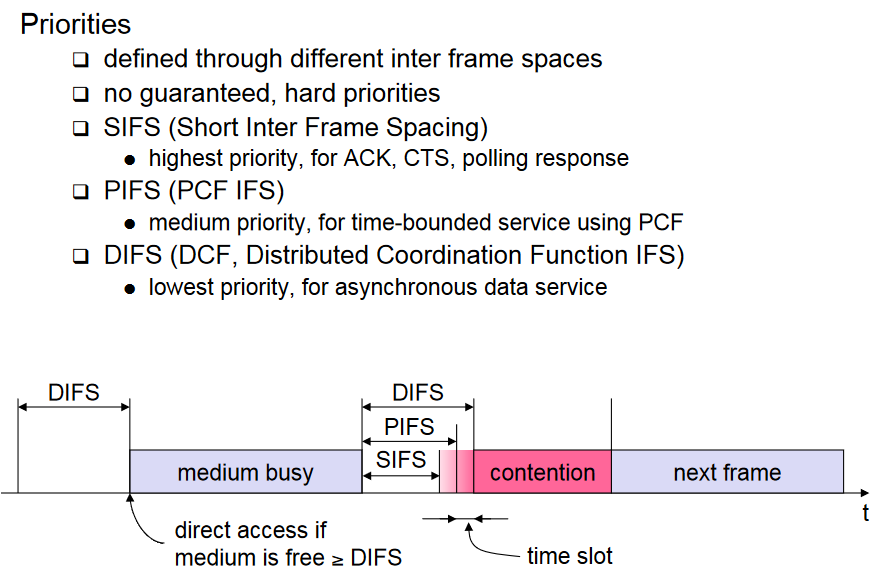
\includegraphics[height=2.5cm]{images/mod-b-slide-16.png}
  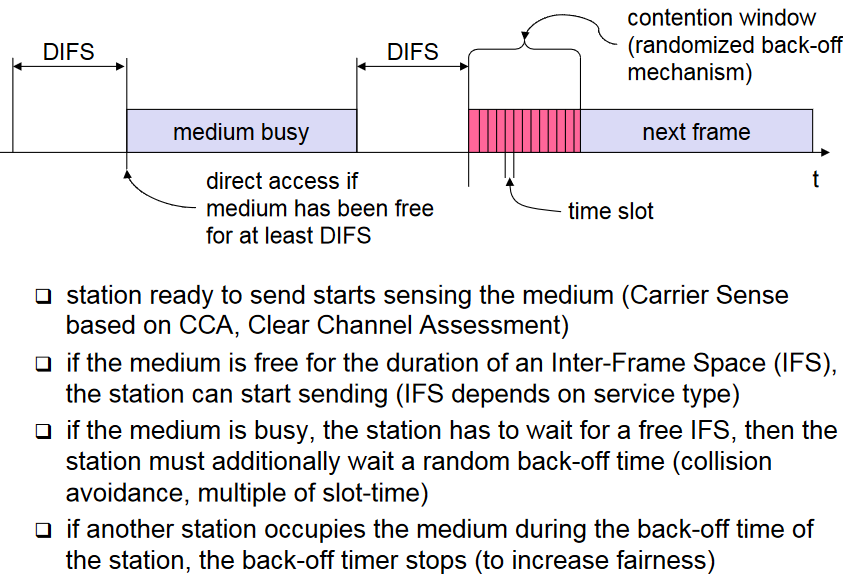
\includegraphics[height=2.5cm]{images/mod-b-slide-17.png}
  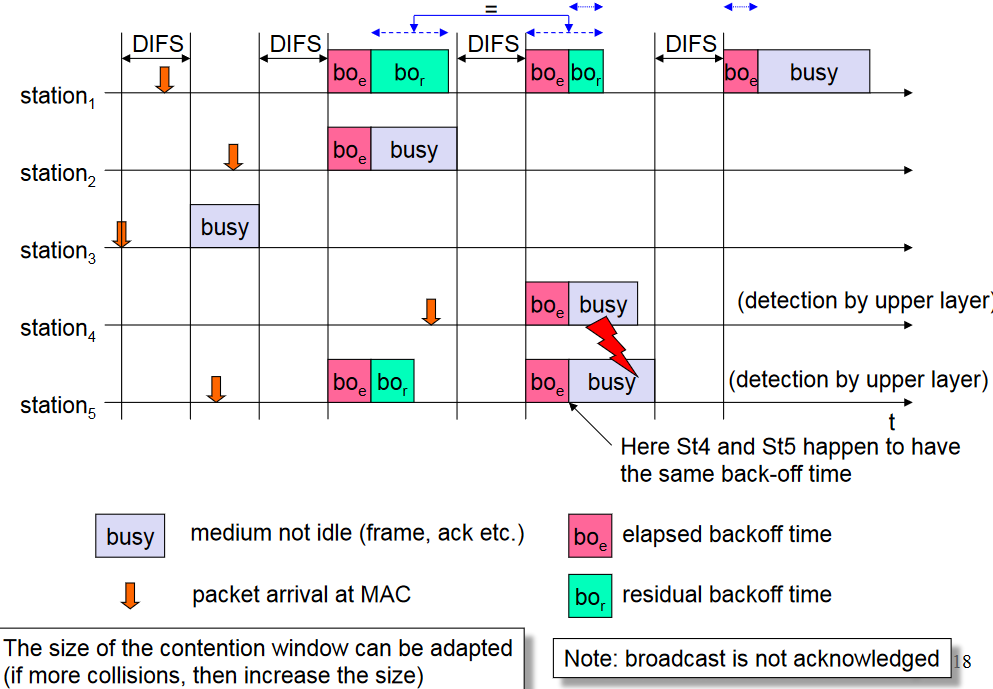
\includegraphics[height=2.5cm]{images/mod-b-slide-18.png}
  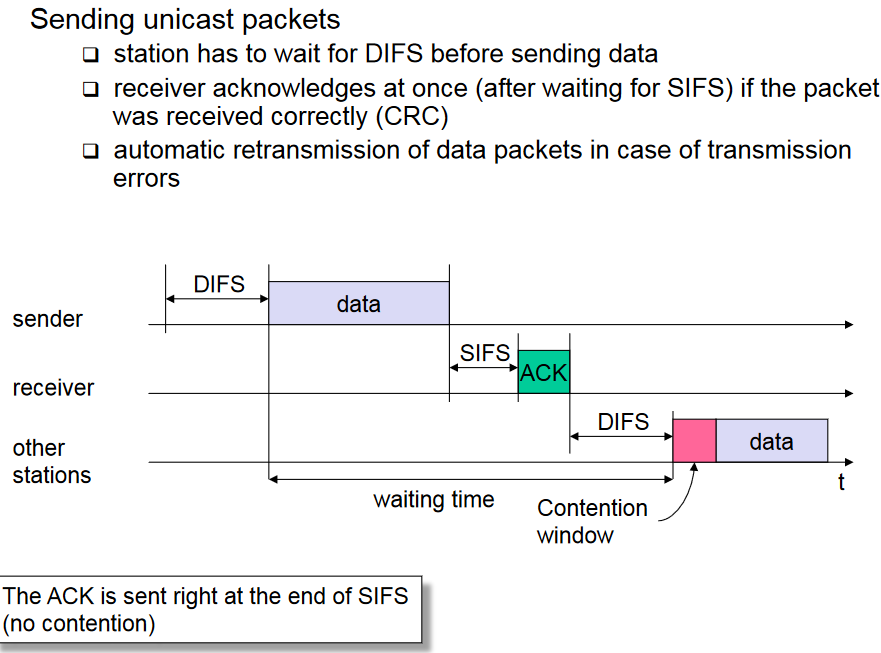
\includegraphics[height=2.5cm]{images/mod-b-slide-19.png}
  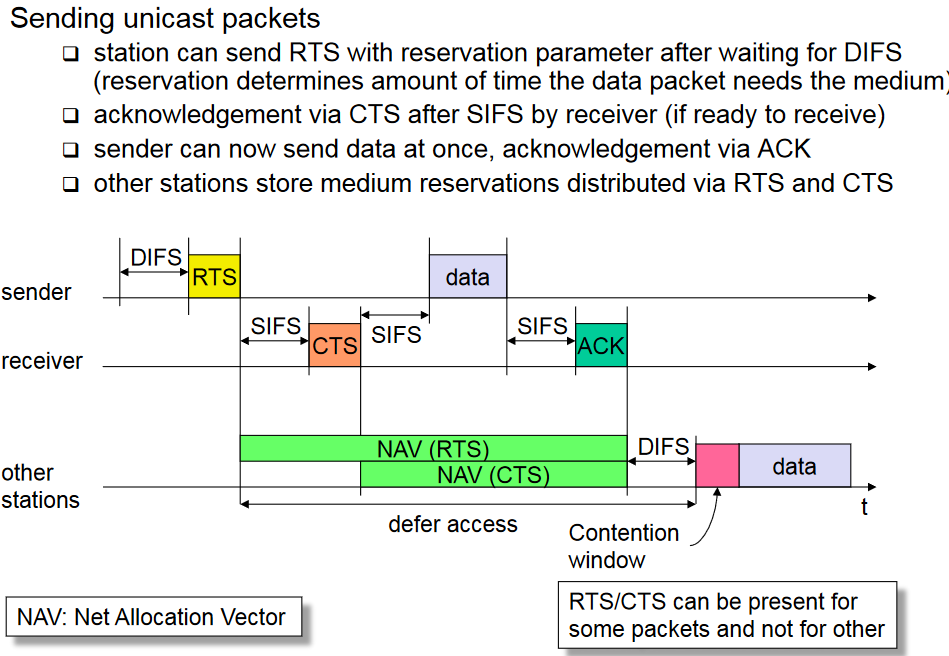
\includegraphics[height=2.5cm]{images/mod-b-slide-20.png}
  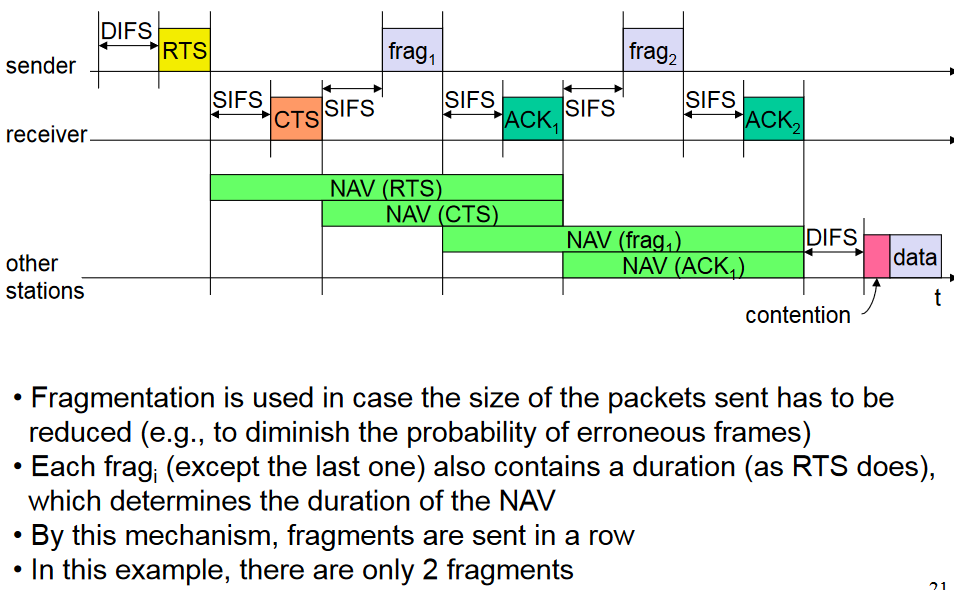
\includegraphics[height=2.5cm]{images/mod-b-slide-21.png}
  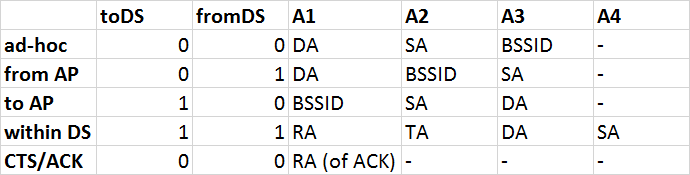
\includegraphics[width=6cm]{images/mod-b-tab-addr.png}
\end{colfig}


\section{Module C}
Proba collision: $p = 1-(1-\pi)^(N-1)$ \\
Proba of transmission: $\pi = \frac{2}{1+W_{min}+pW_{min}\sum\limits_{k=0}^{m-1}(2p)^k}$\\
\subsection{DOMINO}
AttX; Attack X, A: attacker, V: victim\\
Att1: A creates collision with source data and receiver CTS/ACK to force it to reduce its rate (if TCP). Detec: Retransmission rate of A $<<$ Vs\\
Att2: Advertised NAV larger than should be: A get more channel use. Detec:repeated pattern of oversized NAVs.\\
Att3: A uses smaller DIFS to have priority. Detec:Smaller DIFS indicates cheater\\
Att4: A uses non-rnd backoff. Detec:Compare avg backoff of each station to average backoff of AP.\\
Att5: ... ?....

\section{Module D1 (Free-space)}
$f \cdot \lambda = c = 3 \cdot 10^8 \frac{m}{s}$\\
$P_R = P_TG_TG_R(\frac{\lambda}{4\pi d})^2 [W]$\\
$[W]$ to $[dBm]$:$10\log_{10}(\frac{1000P_R[mW]}{1[mW]})[dBm]$\\
$G_X = \frac{4\pi \eta_X A_X}{\lambda^2}$, $10log_{10}(G_X)[dB]$\\
Parabola: $G_X = \frac{7\pi r_X^2}{\lambda^2}$\\
"Signal level" $= 10log_{10}(\frac{P_R[W]}{1[W]})[dBW]$ \\
$ERP = P_TG_T$, $Loss = \frac{P_T}{P_R}$\\
$N_0 = kT[\frac{W}{Hz}], k = 1.3803 \cdot 10^{-23}[\frac{J}{K}]$\\
Noise in bandwidth of B Hertz: $N = kTB [W]$\\
Energy per bit [J]: $E_b = \frac{P_R[W]}{Rate[bits/s]}$\\
Optical LOS: $d = 3.57\sqrt{h}$
Effective LOS: $d = 3.57\sqrt{Kh}, K=4/3$\\
d: dist antenna - horizon [km], h: antenna height [m]\\
Max dist between 2 antennas for LOS propagation: $3.57(\sqrt{Kh_1}+\sqrt{Kh_2})$

\section{Module D2}
Cluster size: $N = i^2 +ij + j^2, i,j=0,1,2,...$\\
Co-channel reuse ratio: $Q = \frac{D}{R} = \sqrt{3N}$\\
D: dist. to center of nearest co-channel cell
$SIR = \frac{S}{\sum\limits_{i=1}^{i_0}I_i}$, S: power of desired signal, $I_i$:interference power caused by the ith interfering co-channel BS, $i_0$: \# of co-channel interfering cells\\
Transmit power of each BS is equal and $\alpha$ is the same throughout the coverage area, then $\frac{S}{I} = \frac{R^{-\alpha}}{\sum\limits_{i=1}^{i_0}D_i^{-\alpha}}$. Considering only the first layer of BS (i.e. all at dist D): $\frac{S}{I}= \frac{R^{-\alpha}}{i_0} = \frac{(3N)^{\frac{\alpha}{2}}}{i_0}$\\
Approx. for corner of cell: $\frac{S}{I} = \frac{R^{-\alpha}}{2(D-R)^{-\alpha}+2D^{-\alpha}+2(D+R)^{-\alpha}}$\\
Radio capacity of cellular network: $m = \frac{B_t}{B_c N} = \frac{B_t}{B_c \frac{Q^2}{3}}$ radio channels/cell. $B_t$: total bandwidth for the system. $B_c$: channel bandwidth. To improve capacity: cell splitting, sectoring.\\
\section{Module E}
\subsection{}


\section{Module F}
\subsection{}


\section{Module H1}
\subsection{}


\section{Module H2}
\subsection{}

\end{multicols*}
\end{document}$